\documentclass{article}
\usepackage[utf8]{inputenc}
\usepackage{hyperref}
\usepackage{graphicx}
\usepackage{subcaption}
\usepackage{cite}
\usepackage{float}
\usepackage{etoc}
\usepackage{blindtext}


%quote
\usepackage{epigraph}
\setlength\epigraphwidth{0.505\textwidth}
\setlength\epigraphrule{0pt}

% margins
\usepackage[a4paper, total={6in, 10in}]{geometry}

% spacing
\setlength{\parindent}{0em}
\setlength{\parskip}{1em}

% fonts (the same as NIPS 2016)
\renewcommand{\rmdefault}{ptm}
\renewcommand{\sfdefault}{phv}

\title{MapReduce\vspace{-1em}}
\author{Tomáš Vlk (vlktoma5@fit.cvut.cz)}
\date{\today}

\begin{document}

\maketitle

\section*{Úvod}

MapReduce je programovací model používaný pro distribuované paralelní výpočty. Původní návrch pochází z Googlu.

\subsection*{Základní myšlenka}

Základní myšlenkou MapReduce přístupu je distrubuce dat na navzájem nezávislé části. Důsledkem toho lze dosáhnout snadného zpracování v jednotlivých uzlech.\par

Další důležitou myšlenkou MapReduce je zpracovávání dat v místě jejich uložení. Tudíž není nutné zbytečně data přesouvat a je tak dosaženo lepší škálovatelnosti.

Samotný přístup se pak dělí na dvě části:

\begin{enumerate}
\item Mapování
\item Redukce
\end{enumerate}

\section*{Popis částí}

Nyní poskytneneme popis a příklady obou částí MapReduce přístupu.

\subsection*{Mapovací funkce}

Vstupem mapovací funkce je seznam prvků, najehož prvky je následně aplikovaná transformace. Mapovací funkce je bezstavová a příkladem takovéto funkce může například být převod stringů na velká písmena.

\subsection*{Redukční funkce}

Redukční funkce pouze agreguje seznam hodnot, který jí je poskytnut, do obvykle menšího množství hodnot. Příkladem takové funkce může být i jednoduchý součet.

\section*{MapReduce přístup}

MapReduce kombinuje oba přístupy zmíněné výše. První je mapovací funkce, po které následuje shuffle a nakonec reduční funkce. U každé části je uvedený příklad na součtu počtu slov stejné délky.

\subsection*{Mapování}

Vstupem do mapovací funkce je seznam hodnot. Mapovací funkce za něj vytvoří pár <klíč, hodnota>. V případě počítání slov vytvoří pár <délka slova, slovo>.

\subsection*{Shuffle}

Vstupem do shuffle funkce je list párů vytvořených pomocí mapovací funkce. Shuffle je promíchá a předá redukční funkci. Každé redukční funkce dostane páry se stejným klíčem.

\subsection*{Redukce}

Redukční funkce provede agregaci párů se stejným klíčem. V případě počítání slov, redukční funkce pouze sečte výskyty prvků se stejným klíčem.

\begin{figure}[h]
\begin{center}
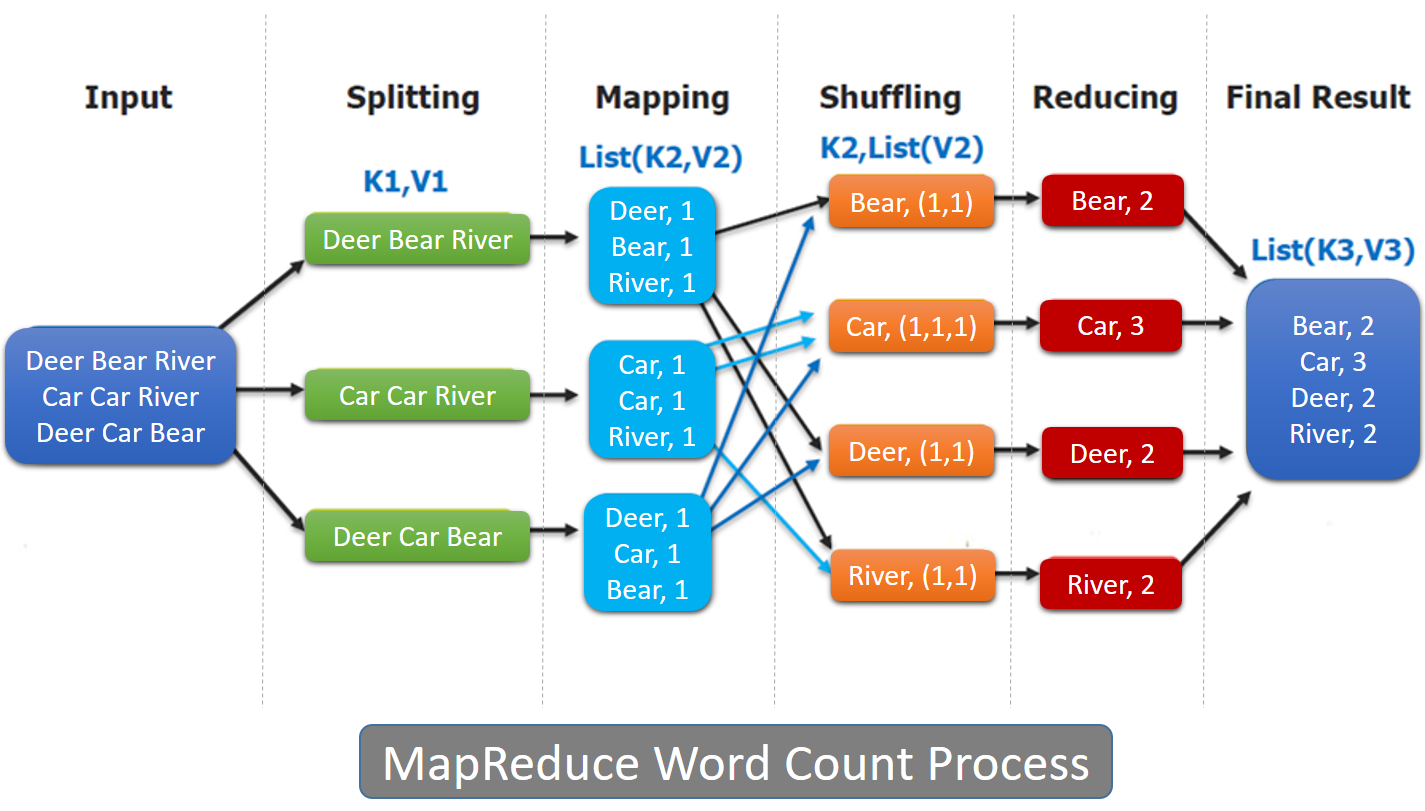
\includegraphics[scale=0.4]{mapReduce.png}
\end{center}
\end{figure}


\section*{Využití}

MapReduce je používaný v Googlu pro generování Google indexu, nebo v Hadoopu ve spojeni s HDFS.


\end{document}
